\chapter{Implementation}\label{s:implementation}

\section{QAS-01 Apply Zero-knowledge proof}
Xiaohui Yang and Wenjie Li\cite{YANG2020102050} state "Zero-knowledge proof (ZKP) is a cryptographic technique,
which means that the prover can convince the verifier that a certain statement is correct without providing the verifier with any additional information or leaking any information about the witness."
The paper shows a method on how to implement Zero-knowledge proof without exposing personal information of the subject. The following scenarios depict a way how the system could respond in a happy flow as in an unhappy flow (hacker).
This method is based on blockchain technology, meaning this scenario can only be executed in online situations.

\graphicspath{ {./images/} }
\begin{figure}[t]
\centering
\caption{Concrete scenarios for QAS-01}
\label{fig:QAS-01}
\end{figure}
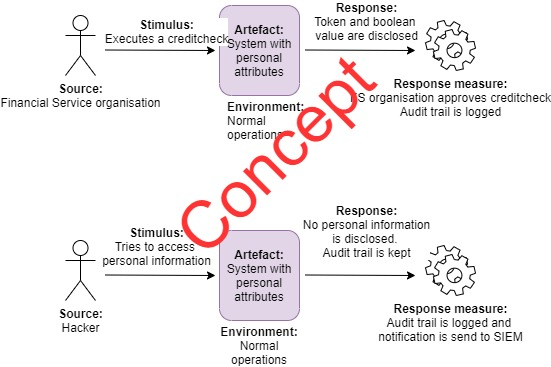
\includegraphics[width=12cm]{QAS-01.jpg}\\

\section{QAS-02 Personal data is minimized to the essentially needed set}

\section{QAS-03 Personal information is shared as a pseudonym}
When it's mandatory to share personal information, because it's for example mandatory by law, it's possible to provide this information as a pseudonym. GDPR \cite{GDPR} defines this method as a possibility to mitigate unwanted disclosure of personal information. 
This technique is already implemented and proven it can work by Erik Verheul \cite{VerheuleID}. 

\section{QAS-04 Transfer of data is encrypted with TLS 1.2 or higher}
A broadly implemented standard. The Dutch government has a reference architecture NORA (Nederlandse Overheid Referentie Architecture) \cite{NORA} which states this standard needs to be applied or otherwise explained why it has not been implemented \cite{NORA_PasToeOfLegUit}. On the part of TLS its clear version 1.2 or higher is accepted, but version 1.3 is prefered \cite{NORA_TLS}. 

%%% Local Variables:
%%% mode: latex
%%% TeX-master: "../thesis"
%%% End:
